\documentclass[9pt]{IEEEtran}

\usepackage[english]{babel}
\usepackage{graphicx}
\usepackage{epstopdf}
\usepackage{fancyhdr}
\usepackage{amsmath}
\usepackage{amsthm}
\usepackage{amssymb}
\usepackage{url}
\usepackage{array}
\usepackage{textcomp}
\usepackage{listings}
\usepackage{hyperref}
\usepackage{xcolor}
\usepackage{colortbl}
\usepackage{float}
\usepackage{gensymb}
\usepackage{longtable}
\usepackage{supertabular}
\usepackage{multicol}

\usepackage[utf8x]{inputenc}

\usepackage[T1]{fontenc}
\usepackage{lmodern}{}
\input{glyphtounicode}
\pdfgentounicode=1

\graphicspath{{./figures/}}
\DeclareGraphicsExtensions{.pdf,.png,.jpg,.eps}

% correct bad hyphenation here
\hyphenation{op-tical net-works semi-conduc-tor trig-gs}

% ============================================================================================

\title{\vspace{0ex}
Kernels}

\author{Marko Medved\vspace{-4.0ex}}

% ============================================================================================

\begin{document}

\maketitle


\section{Part 1}

In this section we implemented the kernelized ridge regression and support vector
regression. In addition to the Linear kernel, we implemented the Polynomial kernel 
and the RBF kernel.

\subsection{Kernelized Ridge Regression Implementation}

This implementation is simple because the fitting algorithm has a closed-form solution:
\[
\boldsymbol{\alpha} = (K_{\text{train}} + \lambda \mathbf{I})^{-1} \mathbf{y}
\]
where \( K_{\text{train}} \) is the kernel matrix computed between training points, and \( \lambda \) is the regularization constant.

Then we can predict with:
\[
\hat{\mathbf{y}} = K_{\text{test, train}} \boldsymbol{\alpha}
\]
where \( K_{\text{test, train}} \) is the kernel matrix computed between the test inputs and the training inputs.




\subsection{Support vector regression implementation}
Here we needed to adapt the Equation 10 from (Smola and Scholkopf, 2004) to a form
 which fits 
the requirements of the \textit{cvxopt.solvers.qp}, that is: 
\[
\begin{aligned}
\text{minimize} \quad & \frac{1}{2} \mathbf{x}^T P \mathbf{x} + \mathbf{q}^T \mathbf{x} \\
\text{subject to} \quad & G \mathbf{x} \leq \mathbf{h} \\
                        & A \mathbf{x} = \mathbf{b}
\end{aligned}
\]
where:
\[
x = \left[ \alpha_1, \alpha_1^*, \alpha_2, \alpha_2^*, \ldots \right]
\]

\vspace{10pt}
\begin{figure}[H]
    \centering
    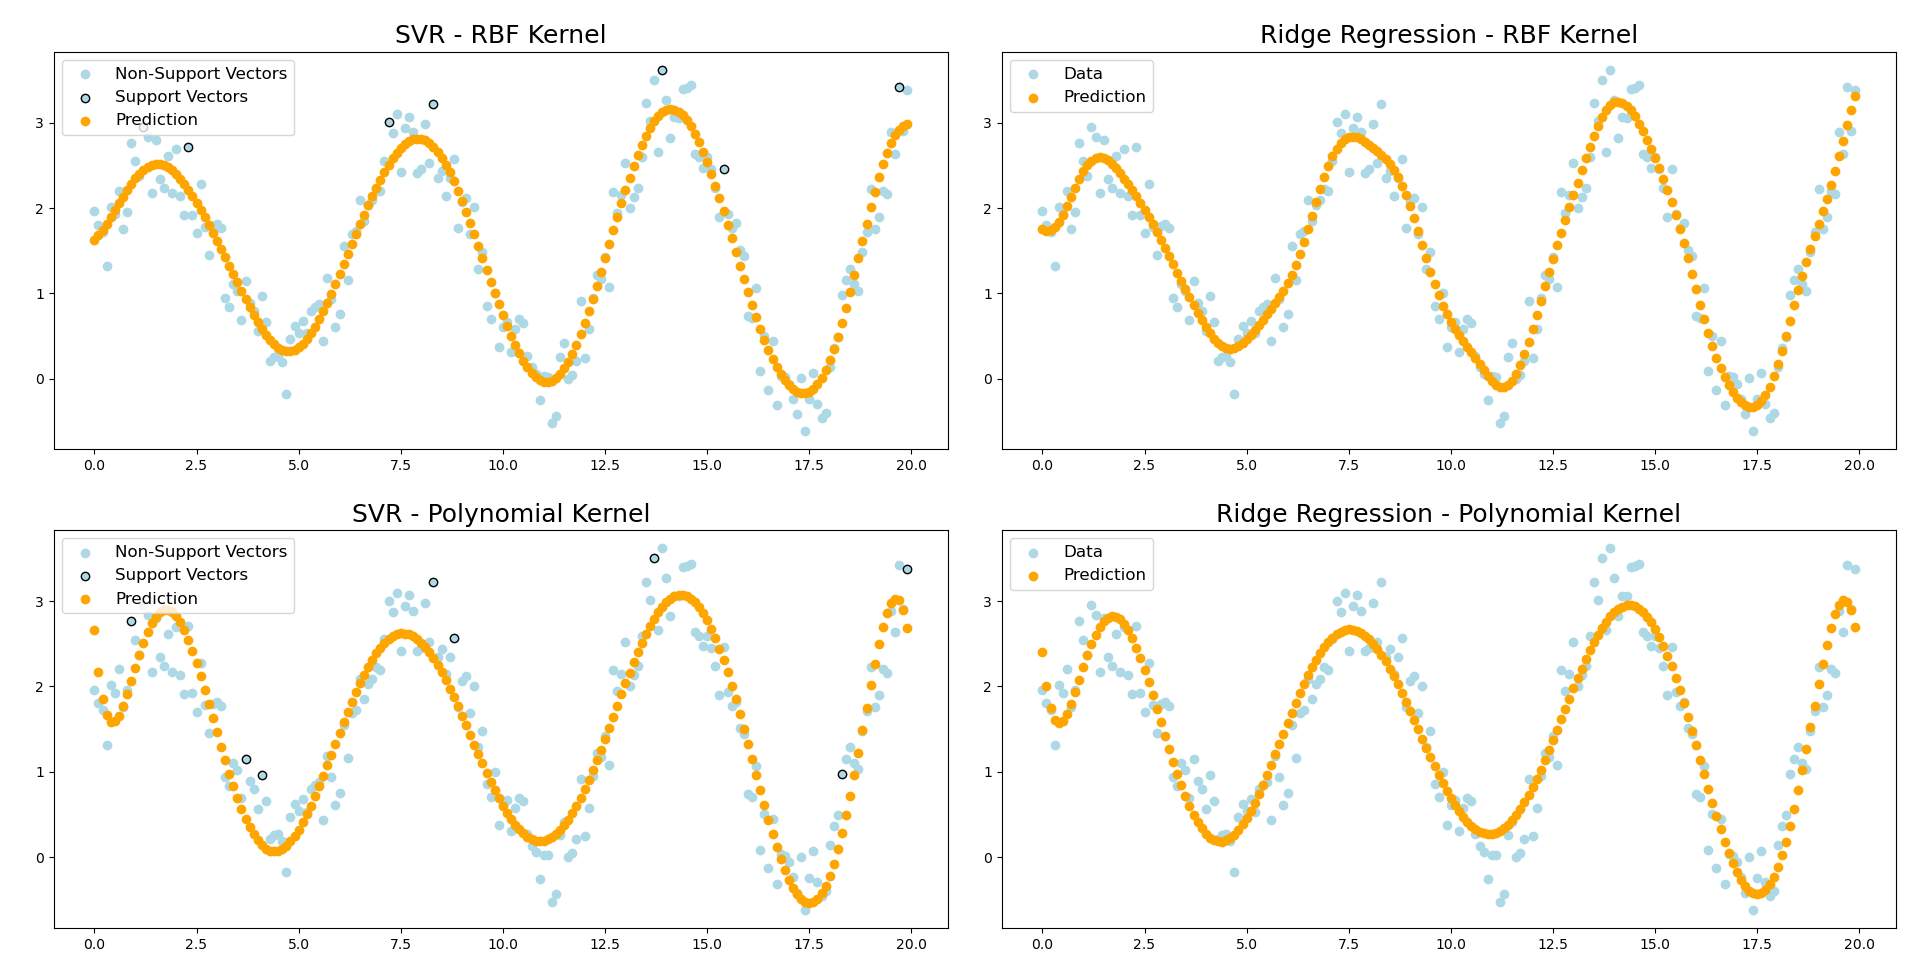
\includegraphics[width=0.9\textwidth]{figures/part1.png}
    \caption{Comparison of SVR and Ridge Regression}
    \label{fig:part1}
\end{figure}


The matrices were calculated as: 
\[
\begin{aligned}
P_{2i,\;2j}   &=\quad k_{ij},\\
P_{2i,\;2j+1} &= -\,k_{ij},\\
P_{2i+1,\;2j} &= -\,k_{ij},\\
P_{2i+1,\;2j+1} &=\quad k_{ij}.
\end{aligned}
\hspace{10pt}
q = 
\begin{bmatrix}
\varepsilon - y_1 \\ 
\varepsilon + y_1 \\ 
\vdots \\ 
\varepsilon - y_n \\ 
\varepsilon + y_n 
\end{bmatrix}
\in \mathbb{R}^{2n}
\]

\[
G = 
\begin{bmatrix}
 -I_{2n} \\ 
 I_{2n}
\end{bmatrix}
\in \mathbb{R}^{(4n) \times (2n)}
\quad
h = 
\begin{bmatrix}
 \mathbf{0}_{2n} \\ 
 C \cdot \mathbf{1}_{2n}
\end{bmatrix}
\in \mathbb{R}^{4n}
\]

\[
A = 
\begin{bmatrix}
 1 & -1 & 1 & -1 & \dots & 1 & -1
\end{bmatrix}
\in \mathbb{R}^{1 \times 2n}
\quad
b = 0
\]
where $K$ is the kernel on the training data, $n$ is the number of data points, 
$\epsilon$ is the margin of tolerance and $C$ is the regularization constant defined 
as $1/\lambda$.\\
We can then predict as: 
\[
\hat{y} = K(X, X_{\text{train}}) \cdot (\boldsymbol{\alpha} - \boldsymbol{\alpha}^*) + b
\]
where b is the bias.


\subsection{Fitting both methods to the 1-dimensional sine data}
We fit both methods, each with both kernels to the 1-D sine data, 
which we can see on Figure~\ref{fig:part1}. Note that the
 support vectors are the data points
  where: \( \alpha_i - \alpha_i^* > 1 \times 10^{-5} \).
   In Table~\ref{tab:parameters} we can see
the parameters we used for each model. Note that for the polynomial kernel to
work, we needed to scale the data.

\begin{table}[h]
\centering
\begin{tabular}{l|l|l}
Model & Kernel & Parameters \\
\hline
SVR & RBF & $\sigma=1$, $\varepsilon=0.5$, $\lambda=0.001$ \\
Ridge Regression & RBF & $\sigma=1$, $\lambda=0.01$ \\
SVR & Polynomial & $M=10$, $\varepsilon=0.7$, $\lambda=0.0001$ \\
Ridge Regression & Polynomial & $M=10$, $\lambda=0.001$ \\
\end{tabular}
\vspace{2pt}
\caption{Parameters for SVR and Ridge Regression.}
\label{tab:parameters}
\end{table}



\newpage
\section{Part 2}
\subsection{Results}
For this part, we applied both methods and kernels to
 the \textit{housing2r} dataset.  
For the polynomial kernel, we evaluated different degrees: \( M \in [1, 10] \).  
For the RBF kernel, we tested a wide range of standard deviations:  
\( \sigma \in \{0.001, 0.01, 0.1, 1, 2, 3, 4, 5, 8, 10, 100\} \). This
 range includes values that produce smoother decision boundaries 
(larger \(\sigma\)) as well as more complex ones (smaller \(\sigma\)).

To assess predictive performance, we used 10-fold cross-validation. 
We considered two strategies for selecting the regularization parameter
 \(\lambda\): a fixed value \(\lambda = 1\), and a data-driven approach 
 using nested cross-validation (with 6 folds in the inner loop) to tune 
 \(\lambda\) for each split.

Uncertainty estimates were computed assuming asymptotic normality of 
the cross-validation results. Specifically, we calculated the standard 
deviation across folds and divided by \(\sqrt{n}\), where \(n\) is 
the number of folds.

To get a somewhat sparse SVR solution, we set \(\epsilon = 5\).  
Figure~\ref{fig:part2} shows the results. Note that with an even larger $\epsilon$ 
the solution could get even more sparse however then the performance started degrading.
 Note that the numbers above and below the 
curves indicate the number of support vectors for each configuration.


\vspace{30pt}
\begin{figure}[H]
    \centering
    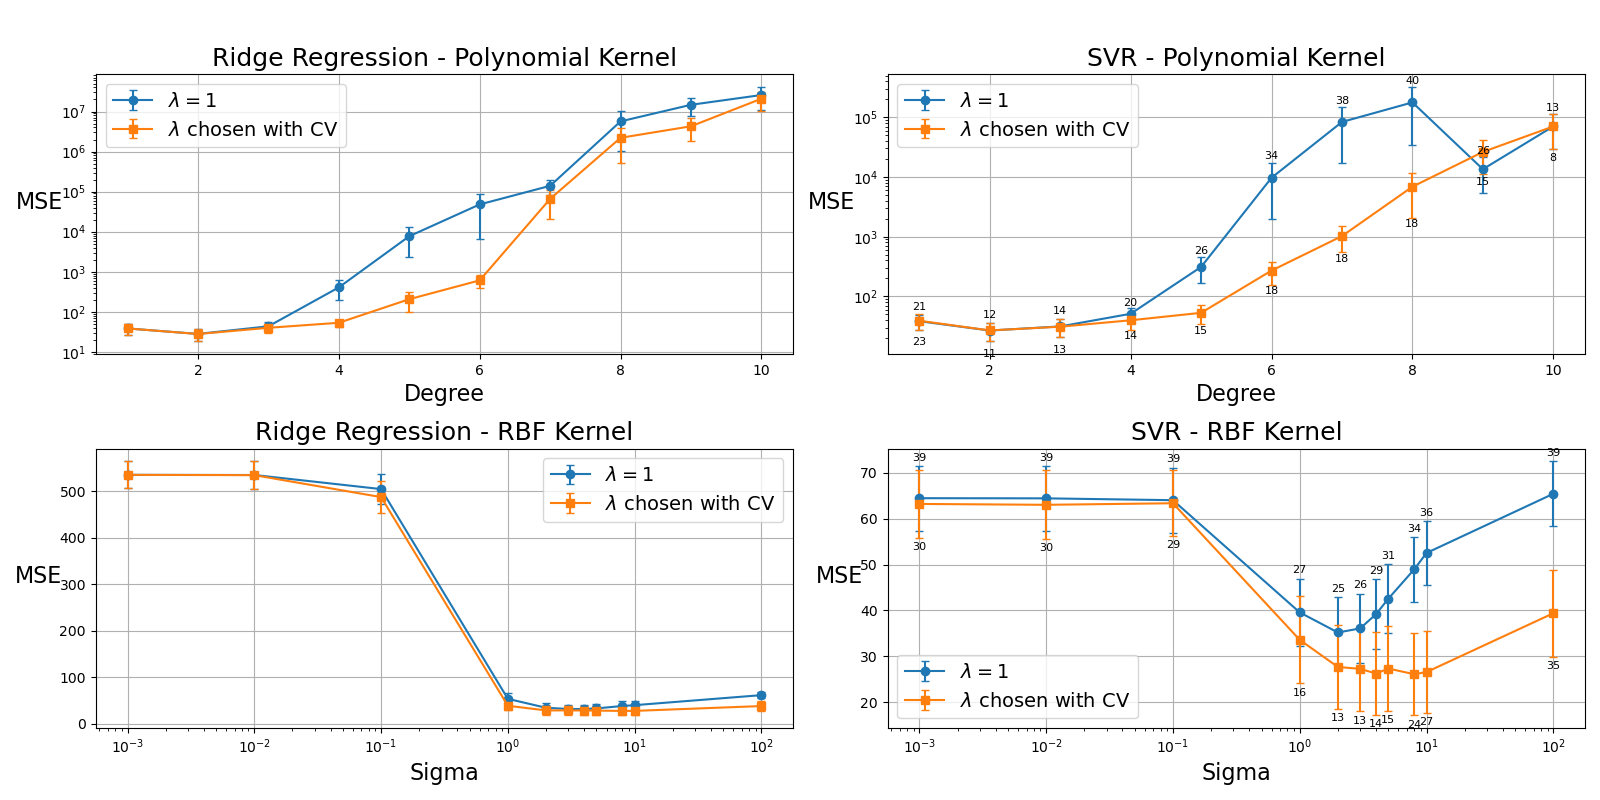
\includegraphics[width=0.99\textwidth]{figures/part2.png}
    \caption{Comparison of models at different parameter values}
    \label{fig:part2}
\end{figure}


\newpage
\subsection{Disscussion}
The first comparison we can draw from Figure~\ref{fig:part2} concerns 
the choice of kernel. The polynomial kernel tends to overfit quickly
 at higher degrees. For both Ridge Regression and SVR, a degree of 2
  gives the best performance. 

The RBF kernel is also quite sensitive to the \(\sigma\) parameter, 
especially for Ridge Regression. Very small \(\sigma\) values lead to 
overfitting and high loss, while values in the range of 1 to 10 yield
 the best results. Larger \(\sigma\) values result in underfitting and 
 worse performance.

Overall, all the models with best chosen parameters
 achieve MSE between 26 and 28, so other factors 
should influence model choice. Ridge Regression benefits from a closed-form 
solution and faster training, making it suitable when training time is 
critical. SVR, on the other hand, requires more training time due to the
 optimization solver, but inference can be faster and more memory-efficient 
 since it relies only on support vectors. For this particular dataset, we pick 
 the Kernelized Ridge regression as the better option. 

Both kernels achieve similar performance (at the best parameters) and yield a comparable number 
of support vectors at their optimal configurations, so either could be a
 suitable choice.

 \newpage
\section{Part 3}
For this part, we used a subset of 1000 images from the UTKFace dataset, which is commonly used 
for age prediction from facial images. All images were resized to $(128 \times 128)$ pixels. 
To evaluate our methods, we performed a train-validation-test split in a 60\%-20\%-20\% ratio.
\\

As a baseline, we used a naive attribute representation where each image is flattened into a 
raw pixel vector. We applied kernelized ridge regression for learning, since it offers significantly 
faster training times compared to SVR. For this baseline, we used the standard
RBF kernel.
\\

In our improved method, we enhanced the RBF kernel by first extracting Histogram of Oriented Gradients (HOG) features from the images, and then computing the RBF kernel on these feature vectors.
\\

Hyperparameter tuning for both methods was performed using grid search. Once the optimal parameters were identified, we retrained the models using the combined training and validation sets. For evaluation, we computed the Mean Squared Error (MSE) on the test set and estimated the uncertainty using asymptotic normality.
\\

The results are shown in Table~\ref{tab:res}. It is evident that the HOG-enhanced representation significantly 
outperforms the naive raw pixel approach.


\vspace{5pt}
\begin{table}[h!]
\centering
\begin{tabular}{lcc}
Representation         & MSE    & Std. Error \\
\hline
Naive attribute representation         & 195.46 & 24.29      \\
HOG-Enhanced representation  & 137.79 & 24.62      \\
\end{tabular}
\vspace{5pt}
\caption{Comparison of the naive attribute representation with our implementation}
\label{tab:res}
\end{table}



\bibliographystyle{IEEEtran}
\bibliography{bibliography}

\end{document}
